% compile with XeLaTeX
\documentclass[dvipsnames,mathserif]{beamer}
\setbeamertemplate{footline}[frame number]
\setbeamercolor{footline}{fg=black}
\setbeamerfont{footline}{series=\bfseries}
\usepackage{tikz}


%\usetheme{Frankfurt}%1
\usetheme{Darmstadt}%1

% for RTL liste
\makeatletter
\newcommand{\RTListe}{\raggedleft\rightskip\leftm}
\newcommand{\leftm}{\@totalleftmargin}
\makeatother

% RTL frame title
\setbeamertemplate{frametitle}
{\vspace*{-1mm}
  \nointerlineskip
  \begin{beamercolorbox}[sep=0.3cm,ht=2.2em,wd=\paperwidth]{frametitle}
    \vbox{}\vskip-2ex%
    \strut\hskip1ex\insertframetitle\strut
    \vskip-0.8ex%
  \end{beamercolorbox}
}
% align subsection in toc
\makeatletter
\setbeamertemplate{subsection in toc}
{\leavevmode\rightskip=5ex%
  \llap{\raise0.1ex\beamer@usesphere{subsection number projected}{bigsphere}\kern1ex}%
  \inserttocsubsection\par%
}
\makeatother

% RTL triangle for itemize
\setbeamertemplate{itemize item}{\scriptsize\raise1.25pt\hbox{\donotcoloroutermaths$\blacktriangleleft$}}

%\setbeamertemplate{itemize item}{\rule{4pt}{4pt}}

\defbeamertemplate{enumerate item}{square2}
{\LR{
    %
    \hbox{%
      \usebeamerfont*{item projected}%
      \usebeamercolor[bg]{item projected}%
      \vrule width2.25ex height1.85ex depth.4ex%
      \hskip-2.25ex%
      \hbox to2.25ex{%
        \hfil%
        {\color{fg}\insertenumlabel}%
      \hfil}%
    }%
}}

\setbeamertemplate{enumerate item}[square2]
\setbeamertemplate{navigation symbols}{}


\titlegraphic {
  \begin{tikzpicture}[overlay,remember picture, opacity=0.1,]
    \node[] at (0, 2.9){
        
\includegraphics[width=0.63\textwidth]{udglogo.png}
  };\end{tikzpicture}}
  \setbeamertemplate{caption}[numbered]
  \begin{document}

  \rightskip\rightmargin
  \title{A Platform for Classifying Melanoma}
  \author{ \Large \textbf{Wilber Eduardo Bermeo Quito} }
  \institute{\large\textbf{Master in Data Science}\\
    ---------\\
    Higher Polytechnic School\\
    ---------\\
  University of Girona}
  \footnotesize{\date{\today }


    \begin{frame}
      \maketitle
    \end{frame}

    \begin{frame}{ Summery}
      \footnotesize \tableofcontents
    \end{frame}

    \section{Introduction}



    \begin{frame}
      \large Motivations:
      \begin{itemize}

        \item Enhance AI\footnote{Artificial Intelligence.} knowledge.

        \item Automation as way to democratize access to research and AI solutions.

        \item CAD\footnote{Computer-Aided Diagnosis.} system are promising path
          towards medical automation.

      \end{itemize}
    \end{frame}


    \begin{frame}
      \large Objectives:

      \begin{itemize}
        \item Gain expertise in deep learning theory and its real-world
          applications.
        \item Explore and study the optimal approach for utilizing the distribution
          of dermoscopy images from the dataset during the training process.
        \item Propose and train deep learning models using transfer learning on ISIC\footnote{Skin Imaging Collaboration.}
          Challenge melanoma images.
        \item Create a CAD infrastructure with trained models, a user-friendly
          web UI\footnote{User Interface.}, a HTTP API\footnote{Application
          Programming Interface.}, and Docker support for easy deployment on
          Linux systems.
      \end{itemize}
    \end{frame}

    \section{Domains}

    \begin{frame}

      \large Problem:

    \end{frame}

    \begin{frame}

      \large Ethical Concern:

    \end{frame}


    \begin{frame}

      \large Regulatory Framework:


    \end{frame}


    \begin{frame}

      \large Solution:

    \end{frame}


    \begin{frame}

      \large Tools:

    \end{frame}



    \section{Data}

    \begin{frame}

    \end{frame}


    \section{Modeling}
    \begin{frame}
      \footnotesize
      The TS fuzzy model can be justified by:
      \begin{itemize}
        \item Its simplicity
        \item Uncertainties
        \item Its acceptable accuracy
        \item ....
      \end{itemize}
      \pause
      \quad \\
      The system can be modeled as:
      \begin{equation*}
        \left\{\begin{array}{l}
            { }^C D^\alpha x(t)=f(x(t),x(t-\tau(t)),u(t)),\, t \geq 0, \\
            x(s)=\varphi(s),\, s \in[-\tau, 0]
        \end{array}\right.
      \end{equation*}
      $x(t) \in \Re ^{n}$ the system state\\
      $u(t) \in \Re ^{m}$ the control vector \\
      $\tau$: the delay
    \end{frame}

    \section{Results}

    \begin{frame}
      \footnotesize
      System behavior without controller
      \begin{figure}[H]
        \centering
        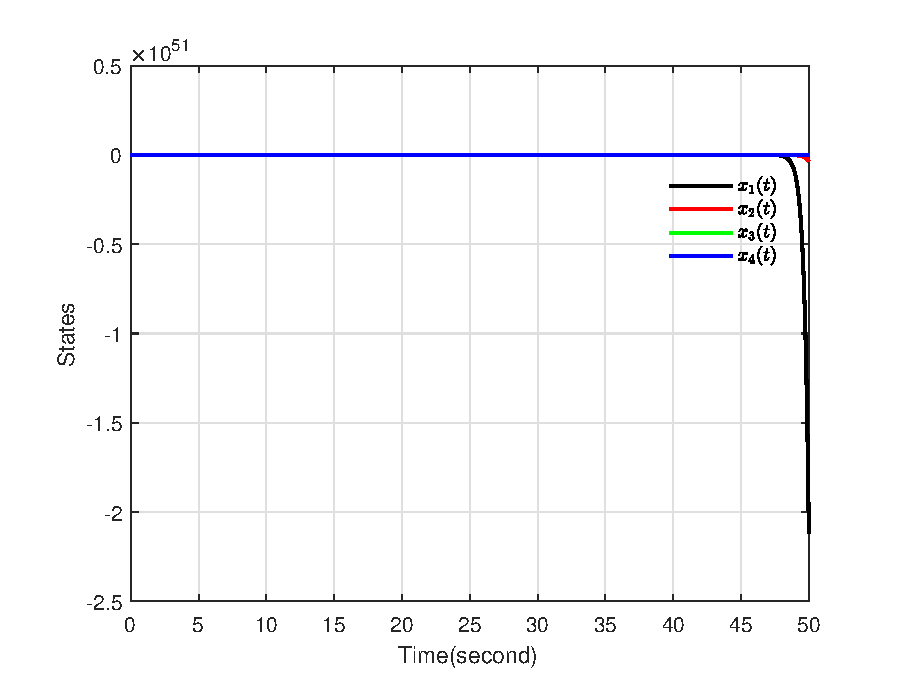
\includegraphics[width=0.75\textwidth]{x_1.eps}
        \caption{System state}
      \end{figure}
      System unstable
    \end{frame}

    \begin{frame}
      System behavior with controller

      \begin{figure}[H]
        \centering
        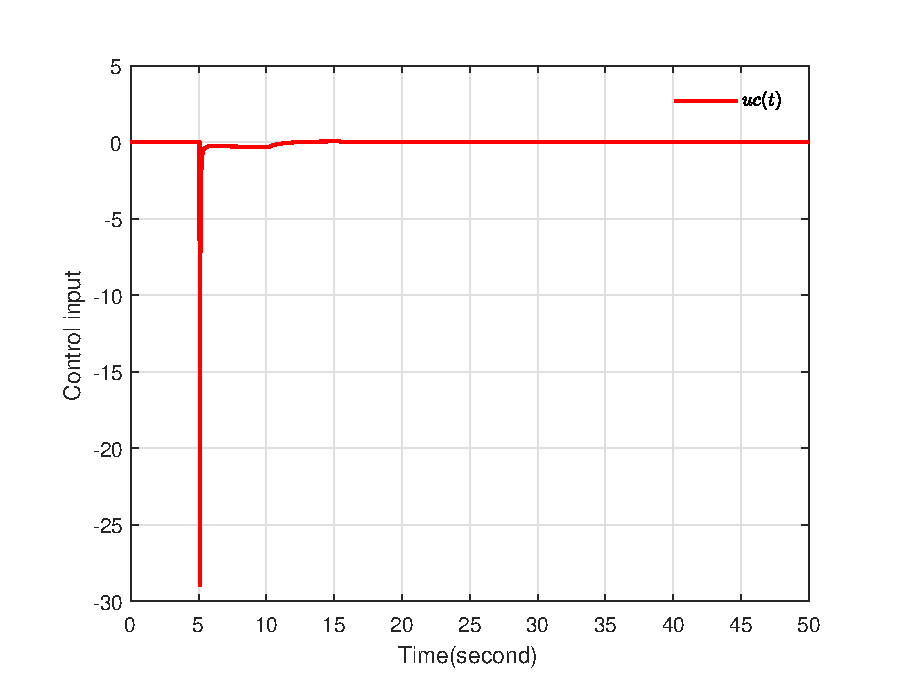
\includegraphics[width=0.75\textwidth]{kuc.eps}
        \caption{Control signal }
        \label{fig3.3}
      \end{figure}
    \end{frame}
    \begin{frame}
      System behavior with controller
      \begin{figure}[H]
        \centering
        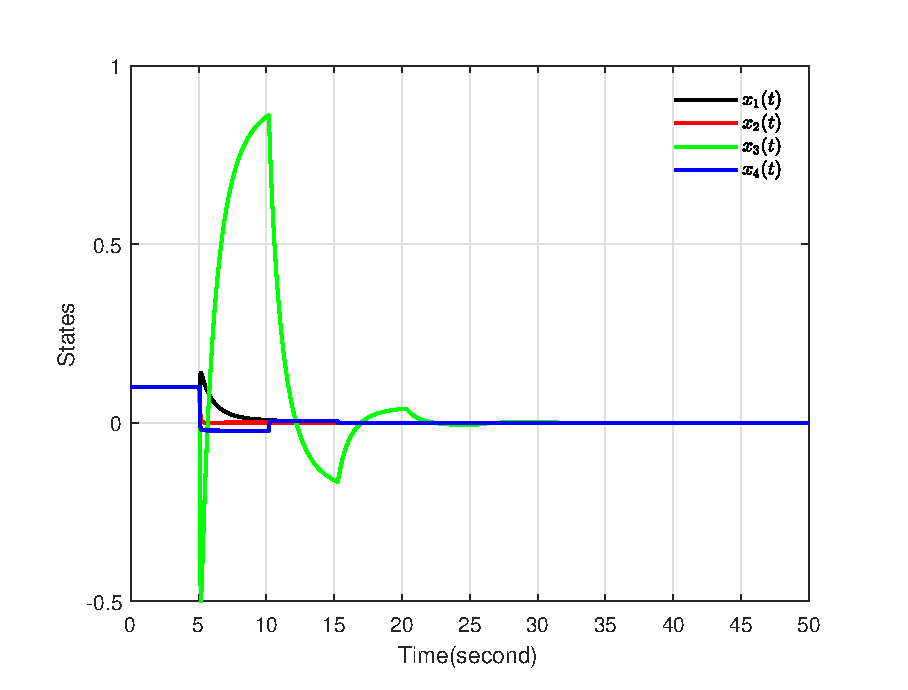
\includegraphics[width=0.75\textwidth]{kstates.eps}
        \caption{System state}
        \label{fig3.4}
      \end{figure}

      The system is stable but it needs more enhancement
    \end{frame}


    \begin{frame}
      System behavior with the proposed controller
      \begin{figure}[H]
        \centering
        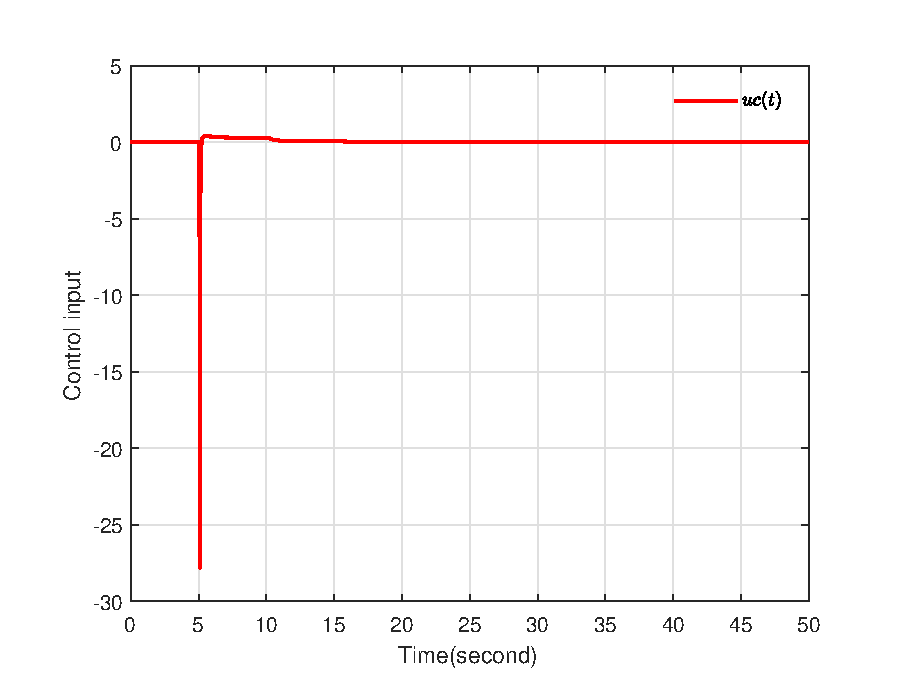
\includegraphics[width=0.75\textwidth]{2uc.eps}
        \caption{Proposed controller signal }
        \label{fig3.5}
      \end{figure}
    \end{frame}
    \begin{frame}
      System behavior with the proposed controller

      \begin{figure}[H]
        \centering
        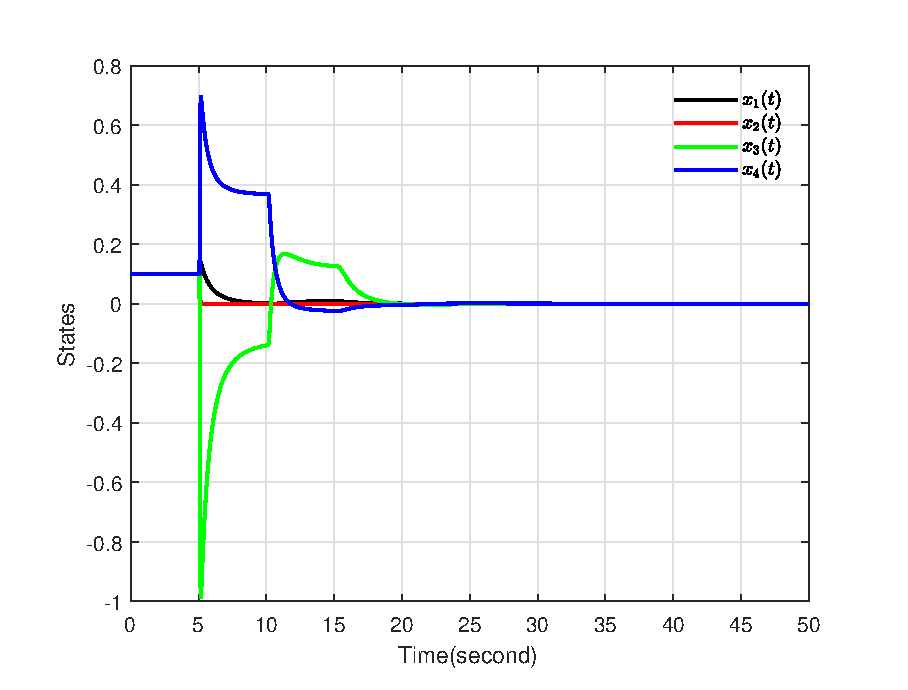
\includegraphics[width=0.75\textwidth]{2states.eps}
        \caption{System state with the proposed controller }
        \label{fig3.6}
      \end{figure}

      \textcolor{blue}{ Stability + better performance}

    \end{frame}

    \begin{frame}
      \footnotesize
      Quantification of the comparative study
      \begin{table}[h]
        \centering
        \begin{tabular}{|*{4}{c|}}
          \hline
  & Classical controller & Proposed controller & Enhancement rate \\
  \hline
          Settling time & $26$  &  $20$ & 23 \% \\
          \hline
          Pic to pic $x_3$  &$1.36$ & $1.16 $ &15 \% \\
          \hline
          $\int\limits_0^{ts}(x_3^2)dt $
                            & $2.5540$ & $0.7771$& 70 \% \\
                            \hline
          $ \int\limits_0^{ts}(u^2)dt$ & $12.8476$ & $7.1868$& 40 \% \\
          \hline
        \end{tabular}
        \caption{Quantification of the comparative study}
      \end{table}
      We remark that
      \begin{itemize}
        \item \textcolor{blue}{\textbf{Enhancement of the settling time of $23\%$}}
        \item \textcolor{blue}{\textbf{ Reduction of the control energy by $40\%$}}
        \item \textcolor{blue}{\textbf{ Overall enhancement by  $70\%$ }}
        \item \textcolor{blue}{\textbf{ Pic to pic reduction by  $15\%$}}
      \end{itemize}
    \end{frame}

    \section{Conclusion and Perspectives}
    \begin{frame}
      \footnotesize
      We conclude that:
      \begin{block}{Conclusion}
        \begin{itemize}
          \item  \textcolor{blue}{\textbf{Lyapunov method efficiency.}}
          \item \textcolor{blue}{\textbf{Proposed controller leads to better performance.}}
          \item \textcolor{blue}{\textbf{Delayed controller enhances the performance.}}
          \item \textcolor{blue}{\textbf{Proposed approach allows reduction of the control energy.}}
        \end{itemize}
      \end{block}
      As perspectives we propose:
      \begin{block}{perspectives}
        \begin{itemize}
          \item Perspective 1.
          \item Perspective 2.
          \item Perspective 3.
        \end{itemize}
      \end{block}
    \end{frame}


    \end{document}
